\section{Ground Station Image Viewer}
\subsection{Agreed design}

The GUI has been planned to have functions such as auto triggering, image type, resolution type, file path chosen, progress bar, help button, stop and delete. Figure \ref{finalGUI} is the screen shot of the final GUI.

\begin{figure}[!hbtp]
\begin{center}
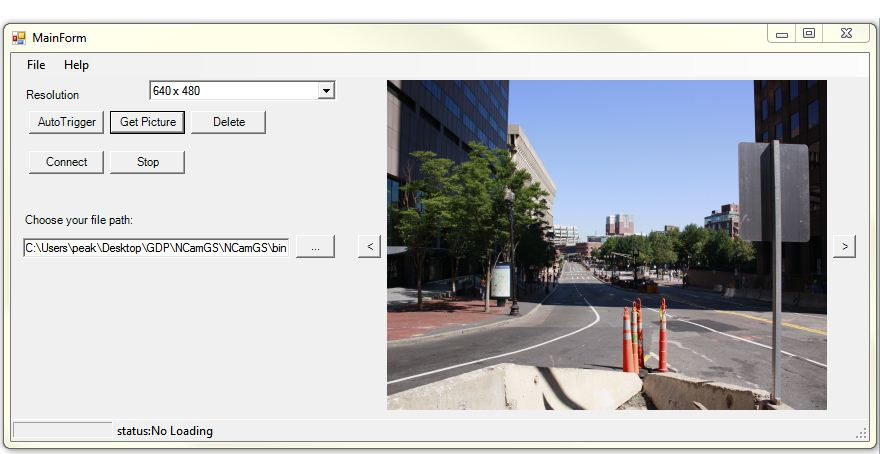
\includegraphics[scale=0.5]{figures/finalGUI.png} 
\end{center}
\caption{final GUI\label{finalGUI}}
\end{figure}
Implementation of the main GUI have omitted some of the buttons in the initial design. 
The gallery button is not needed because the left and right button is use for scrolling the whole directory of the image. 
The top tool strip menu has been added because this layout is familiar to any user. 
The image type have been removed because the raw image data makes the stream data slow and the image viewer program is not supported the file type.
The priority is speed of transmitting the data from the UAV. 
Therefore, raw image is not the option for the user. 
The progress bar has moved to the button left of the page instead of displaying it below the pictureBox.
This allow the application to have bigger picture box, more compact size and more professional looks.
The stop button allows the user to interrupt the downloading image.

\subsection{Agreed Class Diagram}

The class diagram have been implemented very differently from the planned one.
This is because the new plan is to decode it on board and then transmitted to the ground station in JPEG smaller file. 
Therefore, the class JPEG file reader has changed to C code and to be implemented on board. 
The DCT class are not needed anymore because all the calculation will be on board. 
The camera command has taken away as well because the payload will do this  process. 
The painting class use to draw each pixel onto the pictureBox, but it has not been implemented in the final program because of the stated reason.
 
\begin{figure}[!hbtp]
\begin{center}
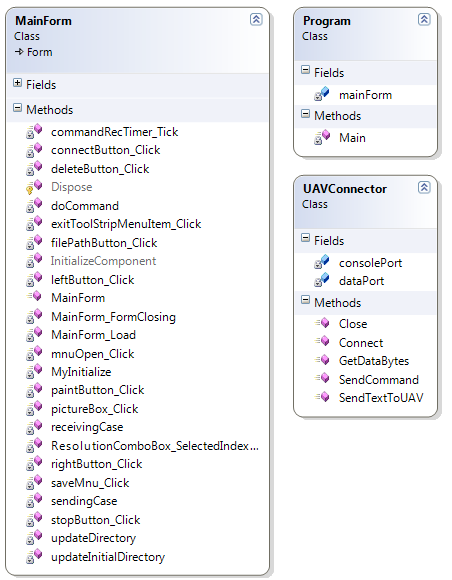
\includegraphics[scale=0.7]{figures/finalClassDiagram.png} 
\end{center}
\caption{Final class diagram of the GUI\label{GUI_finalClassDiagram}}
\end{figure}
\subsection{Agreed Use Case Diagram}
Figure\ref{GUI_finalUseCase} shows an agreed use case diagram. 
It has changed slightly from the initial use case. 
The user does not have to control the data stream, this is because the program was planned to do this automatically during the process of getting picture. 
The type of image can not be chosen because the raw image will be too big and the program can not handle that type of image.

\begin{figure}[!hbtp]
\begin{center}
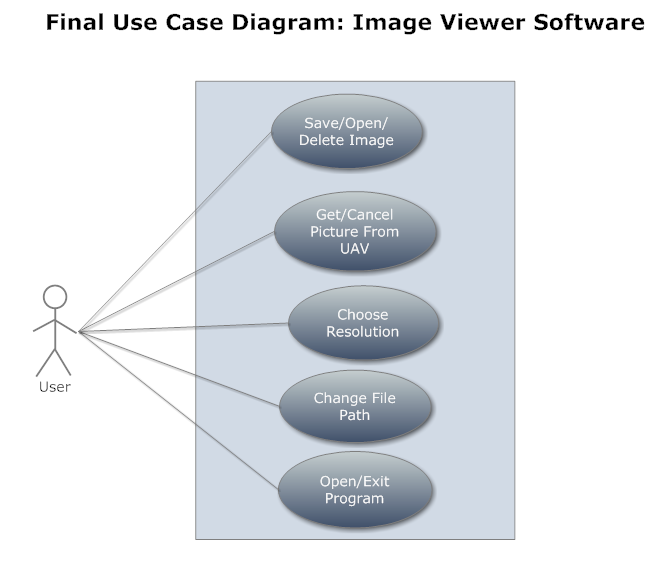
\includegraphics[scale=0.7]{figures/FinaluserCase.png} 
\end{center}
\caption{Final use case diagram of the GUI\label{GUI_finalUseCase}}
\end{figure}

\subsection{.NET C\# class: Socket for the UAV Port Connector}
The socket class was the class chosen for the UAV port connector. 
It support TCP connection between the client and the server to do low level communication work\cite{xiaX}. 
The System.IO.Ports namespace has a SerialPort class that can control settings of the port such as baud rate, stop bit, parity bit, and data length.
However, this become a disadvantage because the baud rate of the UAV has to be fixed according to the specification. 
Although it is good to set up a port, but for the software that uses an existing port, the Socket class is more useful and easier to implement by the programmer. 
The changes of class improve efficiency of connection between port and the program. 
The baud rate and extra bits are automatically adjusted to be the same as the port, so the setting is identical between the input and output.